	
\documentclass[11pt,a4paper]{article}
\usepackage{amsmath}
\usepackage[utf8]{inputenc}
\usepackage{graphicx}	%Grafiken


\title{Abstract of Computer Graphics}
\author{Andreas Ruscheinski \ Christian Delfs}
\date{}
\begin{document}
\maketitle

\section{Introduction}
	\subsection{What is Computer Graphics?}
		\begin{itemize}
			\item deals with all aspect of image creation with computers
		\end{itemize}
	\subsection{Application Areas}
	\subsection{History}
	\subsection{Image formation}
		\begin{itemize}
			\item form images on a two dimensional device analogous how images are formed by physical systems (Cameras and so on)
			\item Objects, Viewer, Light sources with attributes how light interacts with materials in scene, IMPORTEND: independence of object, viewer and light sources
			\item Ray Tracing: follow rays from light with maybe collusions with object to lens (camera) or going to infinity
			\item Luminance Image: Monochromatic (grey levels) like black-white-films
			\item Color Image: perceptional attributes (hue, saturation, lightness)
			\item Additive Color: adding amouts of three primaries (RGB), Monitor
			\item Subtractive Color: form color by filter white light (CYM), Printing
			\item Pinhole Camera: use trigonometry to find project 
			\begin{center}
				\includegraphics[scale=0.3]{pictures/pic1.jpg}
			\end{center}
			\item Synthetic Camera: projection of image on image plane, camera views on image plane ?????
			\item Advantages of SC: separation of objects, viewer, light sources, two-dimensional graphics is a special case of three-dimensional graphics, simple api with fast hardware implementation
			\item cant compute color or shade of each object independently reasons: blocked form light, reflects, translucent
			\item disadvantages of ray tracing: easy calculation for easy object, but on compley objects FUCK UP especially with lights and shadows
		\end{itemize}
	\subsection{Basic Architecture} 
		\begin{itemize}
			\item Physical Approaches: RayTracing = SLOW, can handle global effects; Radiosity: Energy based approaced = MUCH SLOWER
			\item Practical Approaches: process one object at time, can only handle local lightning, pipeline architecture
			\begin{center}
				\includegraphics[scale=0.5]{pictures/pic4.jpg}
			\end{center}
			\item Vertex Processing: much work is converting object representations form one coordinate system to another (Object Coordinates, Camera Coordinates, Screen Coordinates)
			\begin{itemize}
				\item Projection: combines 3D viewer with the 3D objects to produce the 2D image
				\item Perspective Projection: all Projectors meet the center of projection
				\item Parallel Projection: projectors are parallel, center of projection is replaced by a direction of projection
			\end{itemize}
			\item Primitve Assembly: vertices must be collected into geometric objects (line segments, polygons, curves and surfaces)
			\begin{itemize}
				\item Clipping: a real camera cannot see the whole world, objects that are not within this volume are said to be clipped out of the scene
			\end{itemize}
			\item Rasterization: create fragments (potential pixels), fragments have locations in frame buffer, color and depth attributes, vertex attributes are interpolated over objects by the rasterizer
			\item Fragment Processing: fragments are processed to determinate the color of pixel in frame buffer, color determined by texture mapping or interpolation of vertex colors, fragments may blocked by other fragments coloser to camera (hidden surface removal)
			\item Programmiers Interface:
			\begin{itemize}
				\item API
				\item specifiy what we nee to form an image (objects, viewer, light sources, materials), handling input from devices
				\item Object Specification: limited set of primitives (points, line segments, polygons, some surfaces)
				\item Camera Specification: postion of center of lens, orientations, lens, film size, orientation of film plane
				\item Light: different types of lights (point lights, spot light, near and far sources, color properties)
				\item Material: absorption, diffuse, specular
			\end{itemize}
		\end{itemize}
	\subsection{RayTracing}
		\begin{itemize}
			\item follow rays of light from a point source
			\item Problems: rays do not affect what we see, scattering produces many rays; Better: ray casting
			\item Ray Casting: rays goes from view to scene, one ray for one pixel
			\item objects are build from primitives and set operations with other objects
			\item Ray is parametric, Sphere is quadric (quadric is a solution set of quadratic functions), Resulting equations is a entry/exit point or no solution if ray misses
			\item one point is visable if we hit light source form point
			\item in case of reflection follow rays from transmitting surfaces, recursive process
			\item Structure: recursivly, calculate for each ray, find intersection with closet surfaces (need object datebase, complexity of calculation limits of object types), compute lightnig at surface, trace reflected and transmittet rays
			\item stop of procedure if no track amout left (some light will be absorbed at each intersetion with object), ignore rays that go of to infinity (workaround, large absorbing sphere around problem), cout steps
			\item color of pixel is the result of local+reflected+transmitted
			\item Computing Intersections, solve equations with maybe nurmerical methods 
			\item easy calculation with planes
			\item polyhedra build from planes
			\item ray enters at furthest intersection with front facing plane, leaves at closest intersection with back facing planes,
			\item if entry is further away then exit,ray muss miss the polehedron
		\end{itemize}

\section{Basic OpenGL}
	\subsection{Architecture}
		\begin{itemize}
			\item  a platform-independent API (Easy to use,  Close enough to the hardware to get excellent performance)
			\item  Focus on rendering
			\item Relatively stable
			\item Evolution reflect new hardware capabilities (3D texture mapping and texture objects, Vertex programs)
			\item OpenGL Libraries
				\begin{itemize}
					\item OpenGL core library (OpenGL32 - Windows,  GL - most unix/linux systems (libGL.a))
					\item OpenGL Utility Library (GLU) (Provides functionality in OpenGL core but avoids having to rewrite code)
				\end{itemize}
			\item OpenGL Functions
				\begin{itemize}
					\item Primitives (Points, Line Segments, Polygons)
					\item Attributes
					\item Transformations (Viewing, Modeling)
					\item Control (GLUT)
					\item  Input (GLUT)
					\item Query
				\end{itemize}
			\item OpenGL Architecture
			\begin{center}
				\includegraphics[scale=0.3]{pictures/pic2.jpg}
			\end{center}
			\item Software Organization
			\begin{center}
				\includegraphics[scale=0.3]{pictures/pic3.jpg}
			\end{center}
			\item OpenGL is a state machine
			\item OpenGL functions are of two types
				\begin{enumerate}
					\item Primitive generating \\
						(Can cause output if primitive is visible, How vertices are processed and appearance of primitive are controlled by the state)
					\item State changing\\
						(Transformation functions, Attribute functions)
				\end{enumerate}
			\item OpenGL is not object oriented so that there are multiple functions for a given logical function (glVertex3f, glVertex2i, glVertex3dv)
		\end{itemize}
	\subsection{GLUT - OpenGL Utility Toolkit}
		\begin{itemize}
			\item  Provides functionality (Open a window, Get input from mouse and keyboard, Menus, Event-driven)
			\item GLUT function
				\begin{description}
					\item[glutInit] allows application to get command line arguments and initializes system
					\item[gluInitDisplayMode] requests properties for the window (the rendering context) 	
					\item[glutWindowSize] in pixels
					\item[glutWindowPosition] from top-left corner of display 	
					\item[glutCreateWindow] create window with title “simple” 	
					\item[glutDisplayFunc] display callback
					\item[glutMainLoop] enter infinite event loop						
				\end{description}
		\end{itemize}
	\subsection{Simple programs in two and three dimensions}
		\begin{itemize}
			\item  Event Loop
			\begin{itemize}
				\item Note that the program defines a display callback function named mydisplay
				\item Every glut program must have a display callback
				\item The display callback is executed whenever OpenGL decides the display must be refreshed, for example when the window is opened
				\item The main function ends with the program entering an event loop
			\end{itemize}
			\item Objectives
			\item Program Structure \\
				(Most OpenGL programs have a similar structure that consists of	the following functions)
				\begin{itemize}
					\item \textbf{main():} defines the callback functions; opens one or more windows with the required properties; enters event loop (last executable statement)	
					\item \textbf{init():} sets the state variables	(Viewing, Attributes)
					\item \textbf{callbacks:} Display function, Input and window functions
				\end{itemize}
			\item TODO: 06-5 PIC
			\item Coordinate Systems
				\begin{itemize}
					\item The units in glVertex are determined by the application and are called object or problem coordinates	
					\item The viewing specifications are also in object	coordinates and it is the size of the viewing volume that determines what will appear in the image	
					\item Internally, OpenGL will convert to camera (eye) coordinates and later to screen coordinates 	
					\item OpenGL also uses some internal representations that usually are not visible to the application
				\end{itemize}
			\item OpenGL Camera TODO: 06-10 PIC
			\item Orthographic Viewing (In the default orthographic view, points are projected forward along the z axis onto the plane z = 0)
			\item Transformations and Viewing
				\begin{itemize}
					\item In OpenGL, projection is carried out by a projection matrix (transformation)	
					\item There is only one set of transformation functions so we must set the matrix mode first glMatrixMode (GL$\_$PROJECTION)	
					\item Transformation functions are incremental so we start with	an identity matrix and alter it with a projection matrix that gives the view volume \textbf{glLoadIdentity(); glOrtho(...);}
				\end{itemize}
			\item Two- and three-dimensional viewing
				\begin{itemize}
					\item In glOrtho(left, right, bottom, top, near, far) the near and far distances are measured from the camera	
					\item Two-dimensional vertex commands place allvertices in the plane z = 0	
					\item If the application is in two dimensions, we can use the function gluOrtho2D(left, right,bottom,top)	
					\item In two dimensions, the view or clipping volume becomes a clipping window
				\end{itemize}
			\item OpenGL Primitives\\
			(GL$\_$POINTS,
			GL$\_$POLYGON,
			GL$\_$LINES,
			GL$\_$LINE$\_$STRIP,
			GL$\_$LINE$\_$LOOP,
			GL$\_$TRIANGLES,
			GL$\_$QUAD$\_$STRIP,
			GL$\_$TRIANGLE$\_$STRIP,
			GL$\_$TRIANGLE$\_$FAN)
			\item OpenGL will only display polygons correctly that are	
				\begin{description}
					\item[Simple:] edges cannot cross
					\item[Convex:] All points on line segment between two points in a polygon are also in the polygon	
					\item[flat:] all vertices are in the same plane
				\end{description}
			\item RGB-Color (in glColor3f the color values range from 0.0 (none) to 1.0 (all), whereas in glColor3ub the values range from 0 to 255)
			\item Indexed Color (Colors are indices into tables of RGB values Requires less memory)
			\item The color as set by glColor becomes part of the state and will be used until changed (Colors and other attributes are not part of the object but are assigned when the object is rendered)
			\item default: smooth shading (OpenGL interpolates vertex colors across visible polygons)
			\item Alternative: flat shading (Color of first vertex, determines fill color)
			\item glViewport(x,y,w,h) - Values in pixels (screen coordinates)
			\item going to 3D means not much changes\\
			(Use glVertex3*(), Have to worry about the order in which polygons are drawn or use hidden-surface removal)
			\item Das Sierpinski-Dreieck ist ein beschriebenes Fraktal, welches eine selbstähnliche Teilmenge eines Dreiecks ist. Teilt man das Dreieck in vier zueinander kongruente und zum Ausgangsdreieck ähnliche Dreiecke, deren Eckpunkte die Seitenmittelpunkte des Ausgangsdreiecks sind, dann sind die Teilmengen des Fraktals in den drei äußeren Dreiecken skalierte Kopien des gesamten Fraktals, während das mittlere Teildreieck nicht zum Fraktal gehört. Diese Aufteilung des Fraktals in skalierte Kopien kann in den äußeren Teildreiecken rekursiv fortgesetzt werden. 
			This is not an ordinary geometric object and it is neither one- nor two-dimensional. Hausdorff dimension: 1.585	
			\item same in 3D Gasket (Instead of glVertex3f, we can start with a tetrahedron)
			\item Because the triangles are drawn in the order they are defined in the program, the front triangles are not always rendered in front of triangles behind them
			\item TODO PIC !!! 07-21
			\item OpenGL uses a hidden-surface method called the \textbf{z-buffer algorithm} that saves depth information as objects are rendered so that only the front objects appear in the image
			\item z-buffer algorithm
				\begin{itemize}
					\item Use a buffer called the z or depth buffer to store the depth of the closest object at each pixel found so far
					\item As we render each polygon, compare the depth of each pixel to depth in z buffer
					\item If less, place shade of pixel in color buffer and update z buffer
				\end{itemize}
			

		\end{itemize}
	\subsection{Interaction}
		
\section{Three-Dimensional Graphics}
	\subsection{Geometry}
		\begin{itemize}
			\item We will need three basic elements	(Scalars,Vectors,Points)
			\item Coordinate-Free Geometry (two triangles are identical if two corresponding sides and the angle between them are identical $\rightarrow$ Physically, points exist regardless of the location of an arbitrary coordinate system)
			\item \textbf{Scalars} can be defined as members of sets which can be combined by two operations (addition and multiplication) obeying some fundamental axioms (associativity, commutivity, inverses).
			\item physical definition: a \textbf{vector} is a quantity with two attributes (Direction,Magnitude)
				\begin{itemize}
					\item Every vector has an inverse	
					\item Every vector can be multiplied by a scalar	
					\item There is a zero vector	
					\item The sum of any two vectors is a vector
				\end{itemize}
			\item Linear Vector Spaces (Mathematical system for manipulating vectors $\rightarrow$ using operations to make expressions like v=u+2w-3r)
			\item \textbf{Points} are used for Location in space
			\item operations allowed between points and vectors\\ (Point-point subtraction $\rightarrow$ vector, point-vector addition $\rightarrow$ vector)
			\item Affine Spaces = Point + a vector space (Vector-vector addition Scalar-vector multiplication Point-vector addition Scalar-scalar operations)
			\item Lines
				\begin{itemize}
					\item Consider all points of the form $P(\alpha)=P_0 + \alpha$\textbf{d}
					\item Set of all points passing through $P_0$ in direction of the vector \textbf{d}
					\item Parametric Form is more robust and general than other forms Extends to curves and surfaces
						\begin{enumerate}
							\item Explicit: y = mx +h
							\item Implicit: ax + by +c =0
							\item Parametric:\\
							x($\alpha$) = $\alpha x_0$ + (1-$\alpha$)$x_1$ \\
							y($\alpha$) = $\alpha y_0$  + (1-$\alpha$)$y_1$
						\end{enumerate}
					\item If $\alpha >= 0$, then $P(\alpha)$ is the ray leaving $P_0$ in the direction \textbf{d}
					\item If we use two points to define v, then\\
						 P($\alpha$) = Q + $\alpha$ (R-Q)=Q+$\alpha$v =$\alpha$R + (1-$\alpha$)Q\\
						 For $0<=\alpha<=1$ we get all the points on the line segment joining R and Q
				\end{itemize}			
			\item An object is \textbf{convex} iff for any two points in the object all points on the line segment between these points are also in the object
			\item Affine Sums (???)
			\item \textbf{Convex Hull} is the Smallest convex object containing $P_1, P_2, ..... P_n$ formed by “shrink wrapping” points
			\item \textbf{Curves} are one parameter entities of the form P($\alpha$) where the function is nonlinear
			\item \textbf{Surfaces} are formed from two-parameter functions P($\alpha$, $\beta$)	
			\item A \textbf{plane} can be defined by a point and two vectors or by three points
			\item \textbf{Normals}
				\begin{itemize}
					\item Every plane has a vector n normal (perpendicular, orthogonal) to it	
					\item From point-two vector form P($\alpha$, $\beta$)=R+$\alpha$u+$\beta$v, we know we can use the cross product to find\\
					n = u x v and the equivalent form (P($\alpha$)-P)*n=0 	
				\end{itemize}
		\end{itemize}
	\subsection{Representation}
	\begin{itemize}
		\item Lineare Independance: a set of vectors are linearly independent $\leftrightarrow \alpha_{1}v_{1}+\alpha_{2}v_{2}+\alpha_{3}v_{3} +\dots = 0$ iff $\alpha_{1}=\alpha_{2}=\alpha_{3}\dots = 0$ thats mean that no vector can be written in combination with the others
		\item Dimension: in vector space the maximum number of l. independent vectors is fixed and is called the dimension, in an n-dimensional space any set of n linearly independent vectors form a basis, any vector v can be written in combination with basis $v_{1},v_{2},v_{3},\dots,v_{n}$ and $v= \alpha_{1}v_{1}+\alpha_{2}v_{2}+\alpha_{3}v_{3} +\dots+\alpha_{n}v_{n}$ where $\{\alpha_{i}\}$ is unique
		\item  $v= \alpha_{1}v_{1}+\alpha_{2}v_{2}+\alpha_{3}v_{3} +\dots+\alpha_{n}v_{n}$ the list of scalars $\{\alpha_{1},\alpha_{2},\alpha_{3},\dots,\alpha_{n}\} $calls representation of v with respect to the given basis, can be written in row or column
		\item Frames: basis + origin = frame, so a frame determined by $(P,v_{1},v_{2},v_{3})$
		\item every point and vector can be descriped in a frame, Point: $p=[\beta_{1},\beta_{2},\beta_{3}]$, Vector: $b=[\alpha_{1},\alpha_{2},\alpha_{3}]$
		\item 0 for Vector, 1 for Point, Point: $p=[\beta_{1},\beta_{2},\beta_{3},1]$, Vector: $b=[\alpha_{1},\alpha_{2},\alpha_{3},0]$
		\item Why this Shit: all transformations can descriped using 4x4 matrices, effective hardware implementation
		\item How to change coordinate Systems: we can descripe the aiming basis with our current basis 
		\begin{center}
			\includegraphics[scale=0.5]{pictures/basis.jpg}
		\end{center}
		\item Representing one Frame in Terms of the other:
		\begin{center}
			\includegraphics[scale=0.6]{pictures/framechange.jpg}
		\end{center}		
	\end{itemize}
	\subsection{Transformations}
	\begin{itemize}
		\item General Transformations: maps points/vectors to other points/vectors
		\item Translation: move of a point to a new location
		\begin{center}
			\includegraphics[scale=0.5]{pictures/translation.jpg}
		\end{center}
		\item Rotation: easy pattern you can learn if you know $x^{'} = x*\cos(\theta)-y\sin(\theta); x^{'} = x*\sin(\theta)+y\cos(\theta)$ and the rotation variable dosent change
		\begin{center}
			\includegraphics[scale=0.5]{pictures/rotationx.jpg}
			\includegraphics[scale=0.5]{pictures/rotationy.jpg}
			\includegraphics[scale=0.5]{pictures/rotationz.jpg}
		\end{center}
		\item Scaling: expand or contract along each axsis
			\begin{center}
			\includegraphics[scale=0.5]{pictures/scaling.jpg}
		\end{center}		
		\item Reflection: special case of Scaling, negative scaling variables
		\item Inverse: compute inverse matricies of tranformation matricies, using simple oberservation we can reduce this complex step
		\item Concatenation: if we use the same transformation for multiple verticies we can compute a overall transformation matrix using matrix multiplication and use this matrix on all vertices
		\item Rotation about a Fixed Point: Move fixed point to origion, Rorate, move back
	\end{itemize}
	\subsection{Transformations in OpenGL}
	\begin{itemize}	
		\item in OpenGL matrices are part of the state
		\item Different Types:
		\begin{itemize}
			\item Model-View (GL\_MODELVIEW):defines how your objects are transformed (meaning translation,rotation and scaling) in your world coordinate frame
			\item Projection (GL\_PROJECTION): defines the properties of the camera that views the objects in the world coordinate frame. Here you typically set the zoom factor, aspect ratio and the near and far clipping planes.
		\end{itemize}
		\item select with glMatrixMode one matrix for manipulation
		\item CTM (current transformation matrix) is a part of the state, applied to all vertices that pass doen the pipeline
		\item the last descriped operation is first exucuted so. $T+R \neq R+T$
		\item OpelGl hast a model-view and projection matrix in the pipeline which are concatenated togester to form the CTM, manipulate independent by setting the corrent matrix mode TODO: Picture 11:8
		\item Matrix-Stacks: with glPushMatrix() and glPopMatrix()
		\item Model-view Matrix: positioning the camera, build models of objects,
		\item Project matrix: is used to define the view volume and to select a camera lens
	\end{itemize}
	\subsection{Building Models}
	\begin{itemize}
		\item Simple: Build a Mesh with Polygons, Problem: ineffcient and unstructured
		\item Better: look for datastructures that separate the geometry (locations of vertices) from the topology (organizazion of the vertices and edges)
		\item Vertex List: geometry in array, use pointers from the vertices into this array; Problem: Shared edges in a polygon would drawn twice
		\item Edge List: descriping edges with verticies
		\item General Problems with this Approach: many function calls, much more calls if using texture and lightning
		\item OpenGL provides Vertex Arrays that allow us to store ata in the implementation 
		\item glDrawElement on indices would replace all glVertex and glColor calls so we have only one function call
	\end{itemize}
\section{Viewing}
	 \subsection{Classical Viewing}
	\begin{itemize}
		\item basic elements: Objects, viewer with a projection surface, Projectors(from objects to surface)
		\item classival views are based on relationships between them
		\item objects are assumed to constructed from fla principal faces
	\end{itemize}
	\subsubsection{Planar Geometric Projections}
	\subsubsection{prallel}
	\begin{itemize}
		\item multiview orthographic
		\begin{itemize}
			\item projectors are orthogonal to projection surface
			\item projection plan parallel to principal face
			\item front, top, side views
			\item advantages: preserves distance and angles $\rightarrow$ shapes preserved, can be used for measurements
			\item disadvantages: cannot see what object realy looks like because many surfaces are hidden from view
		\end{itemize}
		\item axonometric
		\begin{itemize}
			\item allow projection plane to move realtive to object
			\item classify by how many angles of a corner of a projected cube are the same (none: trimetric, two: dimetric, three: isometric)
			\item advantages and disadvantages: lines are scaled but can find scaling factors, line preserved but angles are not, can see principal faces of box-like object, some optical 				illusions are possible, does not look real
		\end{itemize}
		\item oblique
		\begin{itemize}
			\item arbitrary relationship between projectors and projection plane
			\item advantages and disadvantages: can pick the angles to emphasize a particular face, angles in faces parallel to projection preserved while we ca still see around side, 
			cannot create with simple camera
		\end{itemize}
	\end{itemize}
	\subsubsection{perspective}
	projectors converge at center of projection
	\begin{itemize}
		\item vanishing points: prallel lines on the object converge at a single point in the projection
		\item drawing simple perspectives by hand uses these vanishing points
		\item three-point perspective
		\begin{itemize}
			\item no principal face parallel to projection
			\item three vanishing points for cube
		\end{itemize}
		\item two-point perspective
		\begin{itemize}
			\item on principal direction parallel to projection plane
			\item two vanishing points for cube
		\end{itemize}
		\item one-point perspective
		\begin{itemize}
			\item one principal face parallel to projection plane
			\item one vanishing point for cube
		\end{itemize}
		\item advatages and disadvantages: obejects further from viewer are projected smaler than the same sized objects closer to the viewer, equal distances along a line are not 				projected into equal distances, angles preserved only in planes parallel to the projection plane, difficult to construct by hand
	\end{itemize}

	\subsection{Computer Viewing}
	three aspects implemented in the pipeline: positioning the camera(model-view matrix); selecting a lens(projection matrix); clipping(view volume)
	\subsection{Parallel Rendering}

\section{Projection}
\subsection{Normalization}
\begin{itemize}
	\item convert all projections to orthogonal projections
	\item Why?
	\begin{itemize}
		\item allows for a single pipeline perspective and orthogonal viewin0g
		\item stays in 4D homogeneous coordinates as long as possible $\rightarrow$ retain 3D informations (for hidden-surface and shading)
		\item simplifies clipping
	\end{itemize}
	\item pipeline view: modelview transf. $\rightarrow$ projection transf.  $\rightarrow$  perspective division (4D to 3D) $\rightarrow$  clipping  $\rightarrow$ projection(3D to 2D)
\end{itemize}


\section{Shading}
\begin{itemize}
	\item light-material interactions cause each point to have diffrent color or shade
	\item need to consider: light sources, material properties, location of viewer, surface oriantation
	\item scattering: light strikes surface $\rightarrow$ some scattered, some absorbed $\rightarrow$  scattered light strikes other surface and so on
	\item rendering equation
	\begin{itemize} 
		\item global
		\item includes shadows, multiple scattering from object to object, translucent surfaces
		\item cannot be solved in general, ray tracing is special case for perfectly reflecting surfaces
		\item $I(x,x')=g(x,x')[ \epsilon (x,x')+ \int_s \rho (x,x',x'')I(x',x'')dx'']$
		\begin{itemize}
			\item $I(x,x')$ Intesity of light from $x'$ to $x$
			\item $g(x,x')$ Visibility function between $x$ an $x'$
			\item $\epsilon(x,x')$ Transfer emittance from $x'$ to $x$
			\item $\rho(x,x')$ Scattering term with respect tp direction $x'$ and $x''$
			\item cannot be evaluated analytically
		\end{itemize}
	
	\end{itemize}
	\item local vs global rendering
	\begin{itemize}
		\item correct shading requires global calculation involving all objects and light sources(incompatible with pipeline)
		\item many technics for approximating global effects $\rightarrow$ objects "look right"
	\end{itemize}
	\item light-material interaction
	\begin{itemize}
		\item light strikes object, is partially absorbend and reflected
		\item amount of reflected light determines color and brightness
		\item reflected light scattered in a manner that depends on smoothness and oriantion of the surface
	\end{itemize}
	\item light sources
	\begin{itemize}
		\item difficult to work with, because light comes from all points of the source
		\item point source: model with position and color,  distant source
		\item spotlight: restrict light from ideal point source
		\item ambient light: same amount of light everywhere in scene, can model contribution of many sources
	\end{itemize}
	\item surfaces: smother $\rightarrow$  reflected light is concentrated; rougher $\rightarrow$ light scatters in all directions
	\item phong model
	\begin{itemize}
		\item simple model
		\item components: diffus, specular, ambient
		\item 4 vectors: to source, to viewer, normal, perfect reflector
	\end{itemize}
	\item ideal reflector
	\begin{itemize}
		\item nomal vector is determined by local oriantation, angle of incidence = angle of relection, vectors must be coplanar
		\item $r=2(l*n)n-l$
	\end{itemize}
	\item lambertian surface
	\begin{itemize}
		\item perfectly diffuse reflector
		\item light scattered equally in all directions
		\item amount of light reflected is proportional to the vertical component of incoming light
	\end{itemize}
	\item specular surfaces
	\begin{itemize}
		\item most surfaces are neither ideal diffusers nor perfectly specular 
		\item smooth surfaces show specular highlights due to incoming light being reflected in directions concentrated clos to the direction of a perfect reflection
	\end{itemize}
	\item modeling specular relections: $I_{r} \sim k_s I cos^{\alpha}\phi$, (reflected intensity, ansorbtion coef, incoming intensity, schininess coeff)
	\item shininess coefficient:	values between 5 and 10 give surface that look like plastic, values of a between 100 and 200 correspond to metals
	\item ambient light
	\begin{itemize}
		\item result of multiple interactions between light sources and objects
		\item amount and color depend on color of lights and material properties of objects
	\end{itemize}
	\item distance terms: light from a point source that reaches surface is inversely propotional to the square of the distance
	\item light sources
	\begin{itemize}
		\item in phong model $\rightarrow$ add result of each light source
		\item each light source has seperate diffuse, specular and ambient terms (no physical justification)
		\item separate red, green, blue components
	\end{itemize}
	\item material properties: match light source properties (nine absorbation coefficients, shininess coefficient)
	\item modified phong model
	\begin{itemize}
		\item specular term is problematic, because it requires calculation of new reflection and view vectors for each vertex\\
		$\rightarrow$ approximation using halfway vector (h)
		\item $h=(l+v)/|l+v|$
		\item l, v specified by application, problem is determing n
		\item plane normals: three points $\rightarrow$  $n=(p_2-p_0)\times(p_1-p_0)$
		\item normal to sphere: given by gradient
		
	\end{itemize}
	\item shading in OpenGL
	\begin{itemize}
		\item steps: enable shading and select model; specify normals; specify material properties; specify lights
		\item normals: part of state, usually we want normal to have unit length so calculations are correct
		\item front and back faces: default $\rightarrow$ only front faces are shaded, if two sided lightning $\rightarrow$ both sides are shaded, each side has its own properties
		\item emissive term: simulate light source by giving material emissive component (uneffected by other sources)
		\item transparancy: matrial properties specified as RGBA values (A for transparency)
		\item efficiency: many material changes can affect performance
		\item polygonal shading: calculation done for each vertex, default $\rightarrow$ vertex shades interpolated across the polygon
		\item Gouraud Shading: find avarage normal at each vertex; apply modified phng model; interpolate vertex shades across each polygon\\
			if polygon mesh approximates surfaces with high curvatures $\rightarrow$ may show edges
		\item Phong Shading: find vertex normals, interpolate vertex normals across edges; interpolate edge normals across polygon; apply modified phong model\\
			if polygon mesh approximates surfaces with high curvatures $\rightarrow$ may look smooth; more work (until recently not available real-time systems)
	\end{itemize}
\end{itemize}

\section{Implementation}
	\subsection{Approaches (object vs image space)}
	\subsection{Implementing the pipeline}
	\subsection{Clipping}
		\begin{itemize}
			\item Must clip out primitives that are outside the view frustum
			\item Must find which pixels can be affected by each primitive
			\item Required Tasks
				\begin{itemize}
					\item Clipping
					\item Rasterization or scan conversion
					\item Transformations 
					\item Some tasks deferred until fragement processing
				\end{itemize}
			\item Rasterization Meta Algorithms\\(2 approaches to rendering a scene with opaque objects)
				\begin{enumerate}
					\item For every pixel, determine which object that projects on the pixel is closest to the viewer and compute the shade of this pixel (Ray tracing paradigm)
					\item For every object, determine which pixels it covers and shade these pixels(Pipeline approach; Must keep track of depths)
				\end{enumerate}
			\item Clipping
				\begin{itemize}
					\item 2D: against clipping window
					\item 3D: against clipping volume
					\item easy: line segments polygons
					\item hard: curves and text (Convert to lines and polygons first)
				\end{itemize}
			\item Clipping 2D Line Segments
				\begin{itemize}
					\item Brute force approach: compute intersections with all sides of clipping window
					$\rightarrow$ Inefficient: one division per intersection
					\item Cohen-Sutherland Algorithm:
					\item Idea: eliminate as many cases as possible without computing intersections
					\item Start with four lines that determine the sides of the clipping window
					\item Cases
						\begin{enumerate}
							\item both endpoints of line segment inside all four lines $\rightarrow$ Draw (accept) line segment as is
							\item both endpoints outside all lines and on same side of a line $\rightarrow$ Discard (reject) the line segment
							\item One endpoint inside, one outside $\rightarrow$ Must do at least one intersection
							\item Both outside $\rightarrow$ May have part inside $\rightarrow$ Must do at least one intersection
						\end{enumerate}
					\item Outcodes (For each endpoint, define an outcode $b_0b_1b_2b_3$)//
					TODO: PIC 19-Folie 11
					\item using Outcodes\\
					TODO: PIC 19-Folie 12
						\begin{enumerate}
							\item outcode(A) = outcode(B) = 0 $\rightarrow$ Accept line segment
							\item outcode (C) = 0, outcode(D) $\ne$ 0 $\rightarrow$ Compute intersection
							\item outcode(E) AND (bitwise) outcode(F) (bitwise) $\ne$ 0\\
							(Both outcodes have a 1 bit in the same place, Line segment is outside of corresponding side of clipping window; reject)
							\item GH and IJ: same outcodes, neither zero but logical AND yields zero\\
							(Shorten line segment by intersecting with one of sides of window; Compute outcode of intersection (new endpoint of shortened line segment); Reexecute algorithm)
						\end{enumerate}
				\end{itemize}
			\item Cohen Sutherland in 3D (Use 6-bit outcodes)
			\item Liang-Barsky Clipping
				\begin{itemize}
					\item Consider the parametric form of a line segment
					\item Significantly more efficient than Cohen–Sutherland.
					\item The idea of the Liang-Barsky clipping algorithm is to do as much testing as possible before computing line intersections.
					\item TODO: 19-Folie 19
					\item Can accept/reject as easily as with Cohen-Sutherland
					\item Using values of $\alpha$, we do not have to use algorithm recursively as with C-S
					\item Extends to 3D
				\end{itemize}
			\item General clipping in 3D requires intersection of line segments against arbitrary plane
			\item TODO PIC 19-Folie 22 und 23
			\item Normalization is part of viewing (pre clipping) but after normalization, we clip against sides of right parallelepiped Typical intersection calculation now requires only a floating point subtraction, e.g. is $x > x_{max}$?
			\item Polygon Clipping is not as simple as line segment clipping (clipping a convex polygon can yield at most one other polygon)
			\item One strategy is to replace nonconvex (concave) polygons with a set of triangular polygons (a tessellation)
			\item as a Black Box (Can consider line segment clipping as a process that takes in two vertices and produces either no vertices or the vertices of a clipped line segment)
			\item Pipeline Clipping
				\begin{itemize}
					\item Clipping against each side of window is independent of other sides
					\item TODO: 20-Folie 7
					\item 3D: add front and back clippers (small increase in latency)
				\end{itemize}
			\item Bounding Boxes (Rather than doing clipping on a complex polygon, we can use an axis-aligned bounding box or extent $\rightarrow$ Smallest rectangle aligned with axes that encloses the
			polygon)
			\item TODO: 20-Folie 10
			\item Hidden Surface Removal (The elimination of parts of solid objects that are obscured by others)
				\begin{itemize}
					\item Object-space approach: use pairwise testing between polygons (objects)
					\item Painter’s Algorithm (Render polygons a back to front order so that polygons behind others are simply painted over)
					\item Depth Sort
						\begin{itemize}
							\item Requires ordering of polygons first because ot every polygon is either in front or behind all other polygons
							\item easy cases first, harder later
							\item Easy Cases (can render independently)\\
							(A lies behind all other polygons + Polygons overlap in z but not in either x or y)
							\item Hard Cases\\
							(cyclic overlap + Overlap in all directions but one is fully on one side of the other + penetration)
						\end{itemize}
					\item Back-Face Removal (Culling)
						\begin{itemize}
							\item checks the normal vector of every surface to render and throw away surface whose vector points away from the viewer
							\item 90$^\circ >= \theta$ ($\angle$ normal and vector to viewer)  $>=$ -90$^\circ$
						\end{itemize}
					\item Image Space Approach\\
					(Look at each projector (nm for an n x m frame buffer) and find closest of k polygons)
				\end{itemize}
			\item Scan-Line Algorithm\\
			TODO: 20-Folie 20
			\item Visibility Testing (to Reduce burden on pipeline and traffic on bus)
			\item[$\rightarrow$] Partition space with Binary Spatial Partition (BSP) Tree
				\begin{itemize}
					\item Can continue recursively\\
					Plane of C separates B from A\\
					Plane of D separates E and F
					\item Can put this information in a BSP tree\\
					$\rightarrow$ Use for visibility and occlusion testing
				\end{itemize}
			\item Rasterization (Determine which pixels that are inside primitive specified by a set of vertices and produces a set of fragments)
			\item DDA (Digital Differential Analyzer) Algorithm
				\begin{itemize}
					\item is used for linear interpolation of variables over an interval between start and end point
					\item used for rasterization of lines, triangles and polygons
					\item Line $y=mx+h$ satisfies differential equation\\
					$\frac{dy}{dx}=m=\frac{\Delta y}{\Delta x}=\frac{y_2-y_1}{x_2-x_1}$
					\item Problem: for each x plot pixel at closest y (leads to interrupted lines)
					\item solved: Using Symmetry $\rightarrow$ if m$>$1, swap role of x and y $\rightarrow$ For each y, plot closest x
				\end{itemize}
			\item Bresenham’s Algorithm
				\begin{itemize}
					\item DDA: one floating point addition per step $\rightarrow$ possible to eliminate all fp
					\item consider only $1>=m>=0$ otherwise solved by symmetry
					\item assume pixel centers are at half integers
					\item after written pixel, only two candidates are possible to come next
					\item TODO 21-Folie 9 und 10
					\item For each x, we need do only an integer addition and a test\\
					$\rightarrow$ Single instruction on graphics chips
				\end{itemize}
			\item Polygon Scan Conversion (Fill)
			\item Winding Number is used to check whether a Point is inside or outside of a Polygon\\
				(inside if winding number $\ne$ 0)
			\item Filling in the Frame Buffer (at end of pipeline)
				\begin{itemize}
					\item Convex Polygons only
					\item Nonconvex polygons assumed to have been tessellated
					\item Shades (colors) have been computed for vertices (Gouraud shading)
					\item Combine with z-buffer algorithm (March across scan lines interpolating shades; Incremental work small)
				\end{itemize}
			\item \textbf{Flood Fill} (can be done recursively if we know a seed point located inside (WHITE)and scan convert edges into buffer in edge/inside color
			(BLACK) $\rightarrow$ determines the area connected to a given node)
			\item \textbf{Scan Line Fill} speeds up Flood Fill by filling lines. Instead of pushing each potential future pixel coordinate on the stack, it inspects the neighbour lines (previous and next) to find adjacent segments that may be filled in a future pass; the coordinates (either the start or the end) of the line segment are pushed on the stack. In most cases this scanline algorithm is at least an order of magnitude faster than the per-pixel one.
			Efficiency: each pixel is checked once.
			\item Antialiasing by Area Averaging (Color multiple pixels for each x depending on coverage by ideal lineg)
			\item Aliasing problems can be serious for polygons (Jaggedness of edges + Small polygons neglected)
		\end{itemize}
	\subsection{Polygon Fill}
	
\section{Discrete Methods}
	\subsection{Buffers}
	\subsection{Bitmaps and Pixel Maps}
	\subsection{Texture Mapping}
	\begin{itemize}
		\item GPU can render 10 millio polygons per second, not enough for clouds, grass, terrain or skin
		\item Example Modeling an Orange: start with orange sphere (to simple), replace sphere with a more complex shape (dimpels usw) $\rightarrow$ a lots of more polygons
		\item Better Approach: take picture and scan it and paste it on a sphere (texture mapping), Problem: result is smooth, workaround: bump mapping
		\item Types of Mapping
			\begin{itemize}
				\item Texture Mapping: use image to fill a polygon
				\item Enviroment (reflection mapping): use a picture of the enviroment for texture maps, allows simulation of highly specullar surfaces
				\item Bump Mapping: emulates altering normal vectors during the rendering
			\end{itemize}
		\item Mapping techniques are implemented at the end of the rendering pipeline
		\begin{center}
			\includegraphics[scale=0.7]{pictures/mappingpipeline.jpg}
		\end{center}
		\item simple idea, but map an image to a surface is complicated (3 or 4 coordinate systems involved)
		\item Coordinate Systems:
			\begin{itemize}
				\item Parametric Coordinates: may be used to model curves and surfaces
				\item Texture Coordinates: used to identify points in the image to be mapped
				\item Object or World Coordinates: conceptually where the mapping takes place
				\item Window Coordinates: final image is really produced
			\end{itemize}
		\begin{center}
			\includegraphics[scale=0.5]{pictures/mappingexample.jpg}
		\end{center}
		\item Problem: how to find the maps
		\item Simple Idea: mapping form texture to coordinates to a point of a surface
		\item Better: Backward Mapping
		\item Backward Mapping: given a pixel, we want to know to which on an object it corresponds, given a point on an object we want to know to which point in the texture it corresponds (difficult to find in general)
		\item Two-part mapping: first map the texture to a simple intermediate surface
		\begin{center}
			\includegraphics[scale=0.5]{pictures/cylindermapping.jpg}
		\end{center}
		\item Box Mapping: easy to use with simple ortographic projection, used in enviroment maps
		\begin{center}
			\includegraphics[scale=0.5]{pictures/boxmapping.jpg}
		\end{center}
		\item Second Mapping: map from intermediate object to actual object, normals from intermediate to actual, normals form actual to intermediate, vectors from center if intermediate
		\begin{center}
			\includegraphics[scale=0.5]{pictures/secondmapping.jpg}
		\end{center}
		\item Aliasing: point sampling of the texture can lead to aliasing errors (TODO: explain)
		\begin{center}
			\includegraphics[scale=0.5]{pictures/aliasing.jpg}
		\end{center}
		\item Area Averaging: (TODO: explain)
		\begin{center}
			\includegraphics[scale=0.5]{pictures/areaaveraging.jpg}
		\end{center}
	\end{itemize}

\section{Programmmable Pipelines}
	\subsection{Backgroudn}
	\begin{itemize}
		\item Two Components: Vertex shaders, Fragment shaders
		\item Geometric Data: set of vetices + type (type: point, line,polygon; vertex data: coordinates, normal bector, texutre coordinates, rgba color and so on)
		\item Per-Vertex Ops: vertex location are transformed by the model-view matrix into eye coordinates, nromals must be transformed with the inferve transpose of the model-view matrix
		\item Primitive Assembly: vertices are next to assembled into objects, transformation by projection matrix, clipping (against user defined planes, view volume), perspective diviison, viewport maping
		\item Rasterization: geometric entitites are rasterized into framgment (fragment corresponds to a point on integer grid a displayed pixel), each fragment has a color, possibly a depth value, texture coordinates
		\item Vertex Processor: takes vertices (position attribute, possibly color, openGL state), produces position in clip coordinates and vertex color
		\item Fragment Processor: takes output of rasterizer (fragments), output a fragment, fragments still go through fragments test (hidden surface removal)
		\item Programmable Shaders: replace fixed function vertex and fragment processing by programmable processors called shaders
		\item Modeler: outputs geometric model plus information for the renderer (specs of cam, materials, lights), differnet renders (ray tracer, radiosity)
	\end{itemize}
	\subsection{Shading Languages}
	\subsection{GLSL}
	\begin{itemize}
		\item Vertex Chader Application: moving vertices (morphing, wave motion, fractals), lightning (more realistic models, cartoon shaders)
		\item Fragment Shader Application: per fragment lightning calculation, texture mapping
		\item Vertex Shader Execution Model:
		\begin{center}
			\includegraphics[scale = 0.5]{pictures/shaderexecmodel.jpg}
		\end{center}
		\item Fragment Shader Execution Model
		\begin{center}
			\includegraphics[scale = 0.5]{pictures/fragmentshaderexecmodel.jpg}
		\end{center}
	\end{itemize}
	\subsection{Input and Interaction}
	\begin{itemize}
		\item Graphical Input: devices can be described either by pyhsical properties (mouse, keyboard, trackball) or logical properties (a position, an object identifier), modes (how and when input i obtained): request or event
		\item Devices such as the data teblet return a position directly to the os
		\item Devices such as the mouse, trackball, joystick return incremental inputs (or velocities) to the OS
		\item Logical Devices: cant tell from code, couble be keyboard, file, output from other programm
		\item Graphical Logical Devices: locator (return postion), pick (id of an object), keyboard (string of characters), stroke (array of postions), valuator (floating number), choice (one of n item)
		\item X Window Input: client-server model for network workstations, client: opengl program, graphics server: bitmap display with a pointing device and a keyboard
		\item Input Modes: devices contain a trigger which used to send a signal to the os (button on mouse, pressing or relasing a key), then triggered input devices return information to os (mouse return position, keyboard returns ASCII code)
		\item Request Mode: input provided to programm only when user triggers device 
		\begin{center}
			\includegraphics[scale = 0.5]{pictures/requestmode.jpg}
		\end{center}
		\item Event Mode: each trigger generates an event, put in an event queue which can be examined by the user program
		\begin{center}
			\includegraphics[scale=0.5]{pictures/eventmode.jpg}
		\end{center}
		\item Event Types: resize and expose Window, click one or more buttons on Mouse, move mouse Motion, press or release key Keyboard, Idle: no event
		\item Callbacks: interface for event-driven input, callback function for each type of event which is recordnized by graphics system, user supplied fuction for event
		\item GLUT callbacks:
		\begin{itemize}
			\item glutDisplayFunc: called if window first opend, reshaped, exposed or user decideds it wants to change the display (every programm must have a display callback)
			\item glutMouseFunc: called if mouse event occurs
			\item glutReshapeFunc: called if window is reshaped
			\item glutKeyboardFunc: called if keyboard event occurs
			\item glutIdleFunc: called if no event is in queue (animations and so on)
			\item glutMotionFunc, glutPassiveMotionFunc: called if window was moved????(not sure)
		\end{itemize}
		\item GLUT Event Loop: puts program in an infinite event loop, each pass through glut looks at events in the queue, for each event glut executes the appropriate callback function if one is defined, if no callback is defined for the event, event is ignored
		\item Posting redisplays: many events may invoke the display callback funtion (often called redisplay) better use glutPostRedisplay() which sets flag for redisplay. Glut will check it at the end of the event loop
		\item Animating a Display: start by clearing the window glClear(), problem: drawing of information in the frame buffer is decoupled from the display of its contet, better we can see partially drawn display (only draw what changes)
		\item Double Buffering: instead of one color buffer, we use two
		\begin{itemize}
			\item Front Buffer: display but not written to Back Buffer
			\item Back Buffer: written to but not displayed
		\end{itemize}
		\item request double buffer: glutInitDisplayMode$($GL\_RGB$|$GL\_DOUBLE$)$
		\item at the end of display callback buffers need to be swapped (glutSwapBuffers)
		\item GLUT callbacks is fixed thats mean you cant change to parameters of an function, work around: using of global variables 
	\end{itemize}
	
\section{Curves and Surfaces}
	\subsection{Representation of Curves and Surfaces}
	\begin{itemize}
		\item until now we worked with flat entities such as lines af flat polygons but the world isnt flat so wee need curves and curved surfaces but hardware can only deals with flat entities so we our implementation need to render them to flat primitives
		\item Modeling with Curves: want representation taht is stable, smooth, easy to evaluate,
		\begin{center}
			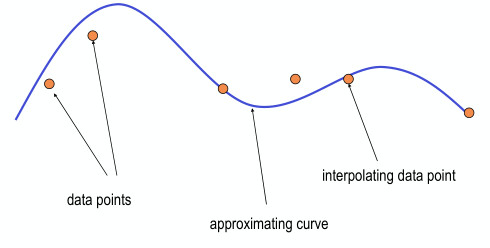
\includegraphics[scale=0.5]{pictures/curves.jpg}
		\end{center}
		\item explicit Representation: Extension from 2d curves ($y=f(x)$) to 3d curves ($y=f(x),z=g(x)$ so that $z=f(x,y)$ defines a surface) but problems with vertical lines and circles
		\item Implicit Representation: two dimensional curve ($g(x,y)=0$) so we can define lines and circles (lines: $a*x+b*y+c=0$ and circles: $x^{2}+y^{2}-r^{2}=0$), in 3d $g(x,y,z)=0$ defines a surface, intersect two surfaces to get a curve, Problem: in general we cannot solve for points taht satisfy equation
		\item Algebraic Surface: $\sum_{i}\sum_{j}\sum_{k}x^{i}*y^{j}*z^{k}=0$, at most 10 Terms, Quadric surface $2 \geq i+j+k$, can solve intersection with ray by reducing problem to solving quadric equation
		\item Parametric Curves: seperate quation for each spatial variable $x=x(u),y=y(u),z=z(u)$ so $p(u)=[x(u),y(u),z(u)]^{T}$ for $u_{max} \leq u \leq u_{min}$ we trace out a curve in two or three dimensions
	\end{itemize}
	\subsection{Bézier Curves and Surfaces}
	\subsection{B-Splines}
\section{Advanced Rendering}
	\subsection{Radiosity}
\section{Hierarchies and Parallel Rendering}
	 \subsection{Traversal Methods}
	 \subsection{Scene Graphs}
	 \subsection{Parallel Rendering}
\end{document}

	